% http://tex.stackexchange.com/a/58828/32098
\newcommand{\gear}[3]{%
  \def\modu{#1}
  \def\Zb{#2}
  \def\AngleA{#3}

  \pgfmathsetmacro{\Rpr}{\Zb*\modu/2}
  \pgfmathsetmacro{\Rb}{\Rpr*cos(\AngleA)}
  \pgfmathsetmacro{\Rt}{\Rpr+\modu}
  \pgfmathsetmacro{\Rp}{\Rpr-1.25*\modu}
  \pgfmathsetmacro{\AngleT}{pi/180*acos(\Rb/\Rt)}
  \pgfmathsetmacro{\AnglePr}{pi/180*acos(\Rb/\Rpr)}
  \pgfmathsetmacro{\demiAngle}{180/\Zb}
  \pgfmathsetmacro{\Angledecal}{(\demiAngle-2*\AnglePr)/2}

  \foreach \zz in{1,2,...,\Zb}{
    \draw
    ({(\zz))/\Zb*360-\Angledecal}:\Rb)
    -- (\zz/\Zb*360-\Angledecal:\Rp)
    to[bend right=\demiAngle]
    (\zz/\Zb*360+\Angledecal:\Rp)
    --
    plot[domain=-0:\AngleT,smooth,variable=\t]
    ({{180/pi*(-\t+tan(180/pi*\t)) +\zz/\Zb*360+\Angledecal}:\Rb/cos(180/pi*\t)})
    % 
    to[bend right=\demiAngle]
    ({{180/pi*(\AngleT+tan(180/pi*-\AngleT)) +(\zz+1)/\Zb*360-\Angledecal}:
      \Rb/cos(180/pi*-\AngleT)})
    % 
    plot[domain=-\AngleT:-0,smooth,variable=\t]
    ({{180/pi*(-\t+tan(180/pi*\t)) +(\zz+1)/\Zb*360-\Angledecal}:\Rb/cos(180/pi*\t)});
  }
}

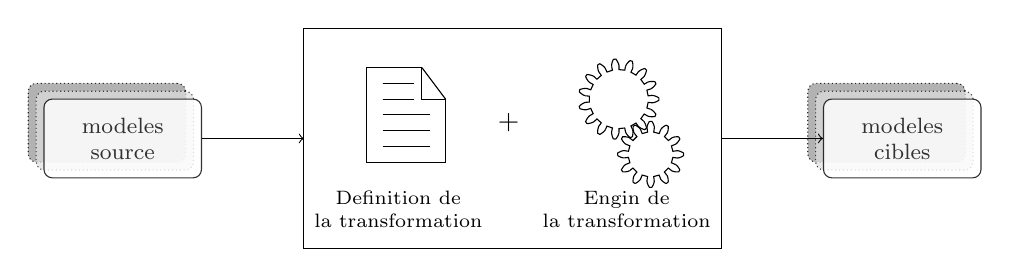
\begin{tikzpicture}

    \begin{scope}[xshift=-3.3cm,yshift=0.5cm]
        \node [densely dotted,minimum height=1cm,fill=gray!75!white,opacity=0.8,minimum width=2cm,draw,rectangle,rounded corners=3pt] {};
        \node [xshift=0.1cm,yshift=-0.1cm,densely dotted,minimum height=1cm,fill=gray!25!white,opacity=0.7,minimum width=2cm,draw,rectangle,rounded corners=3pt] {};
        \node [xshift=0.2cm,yshift=-0.2cm,minimum height=1cm,minimum width=2cm,draw,fill=white,opacity=0.8,rectangle,rounded corners=3pt,font=\footnotesize,align=center] (left) {modeles\\ source};
        \draw[->] (left) -- (2.5cm,-0.2cm);
    \end{scope}
    \begin{scope}[xshift=6.6cm,yshift=0.5cm]
        \node [densely dotted,minimum height=1cm,fill=gray!75!white,opacity=0.8,minimum width=2cm,draw,rectangle,rounded corners=3pt] {};
        \node [xshift=0.1cm,yshift=-0.1cm,densely dotted,minimum height=1cm,fill=gray!25!white,opacity=0.7,minimum width=2cm,draw,rectangle,rounded corners=3pt] {};
        \node [xshift=0.2cm,yshift=-0.2cm,minimum height=1cm,minimum width=2cm,draw,fill=white,opacity=0.8,rectangle,rounded corners=3pt,font=\footnotesize,align=center] (right) {modeles\\ cibles};
    \draw[<-] (right) -- (-2.1cm,-0.2cm);
    \end{scope}
    \draw (-0.8,-1.1) rectangle (4.5,1.7);
    \begin{scope}[scale=1]
        % fichier (http://tex.stackexchange.com/a/174673/32098)
        \draw (0,0) -- (0,1.2) -- (0.7,1.2) -- (0.7,0.8) -- (1,0.8) -- (1,0) -- cycle;
        \draw (0.7,1.2) -- (1,0.8);
        \foreach \y in {0.2,0.4,0.6}{
            \draw (0.2,\y) -- (0.8,\y);
            \draw (0.2,0.8) -- (0.6,0.8);
            \draw (0.2,1) -- (0.6,1);
        }
        \node at (0.4,-0.6) [rectangle,align=center,font=\scriptsize] {Definition de\\ la transformation};
        \node at (1.8,0.5) {$+$};
        \begin{scope}[xshift=3.2cm,yshift=0.8cm,rotate=-60]
            \begin{scope}[scale=0.02]
                \gear{3}{15}{20}
                \begin{scope}[xshift=40.5cm,rotate=180/12]
                    \gear{3}{12}{20}
                \end{scope}
            \end{scope}
        \end{scope}
        \node at (3.3,-0.6) [rectangle,align=center,font=\scriptsize] {Engin de\\ la transformation};
    \end{scope}

\end{tikzpicture}
